\subsection{Direkte Evaluation der Erklärungen}
\label{sec:study_results_qualitativ}

Die zuvor analysierten Metriken betreffen ausschließlich die Auswirkungen von Erklärungen auf die \textit{Objectives} für die Integration - im konkreten Fall \textit{Usage Increase}, \textit{System Acceptance} und \textit{Satisfaction}.

\subsubsection{Ziel der direkten Evaluation}

Mithilfe der Metriken konnte überprüft werden, welche Erklärungen, in welchen Kombinationen den zuvor aufgestellten Anforderungen genügen. Es kann allerdings für die statischen Erklärungen keine Empfehlung abgeleitet werden, da diese insgesamt keine signifikant positiven Auswirkungen haben bzw. warum sowohl positive und negative Effekte im Vergleich zum ausschließlichen Einsatz der \textit{Context}-Erklärungen messbar sind. Folglich ist eine direkte Evaluation der Erklärungen nötig, wie sie auch im Leitfaden vorgeschlagen wird. Insbesondere wird dort empfohlen nicht nur Verhaltensmetriken, sondern auch qualitative Evaluationen von \textit{End Usern} zur Bewertung von Erklärungen zu nutzen. Daher ist im Anschluss an die 

Eine zweite Analyse soll zusätzliche Daten liefern, um die Ergebnisse Einflüsse der integrierten Erklärungen auf andere Qualitätsaspekte besser interpretieren zu können.

Das Ziel ist es folglich, konkrete Probleme oder Verbesserungspotential der entwickelten statischen Erklärungen aufzudecken.

\subsubsection{Methode}

Die direkte Analyse der Erklärungen ist wiederum in zwei Teile gegliedert. Zum einen wurden während der Case Study einige Meta-Daten gesammelt. Es wurde beispielsweise aufgezeichnet, wie viele der \textit{End User}, die die Möglichkeit hatten, auf die statische Erklärungen zuzugreifen, diese genutzt haben und wie lange, sie diese im Fokus hatten.

Um qualitative Aussagen zu den Erklärungen zu erhalten wurde außerdem ein Quasi-Experiment durchgeführt. Bei diesem wurden vier Studienteilnehmern jeweils alle vier Erklärungen gezeigt bzw. sie haben mit diesen interagiert. Im Anschluss an jede Erklärung wurden ihnen die gleichen Aussagen zur Bewertung auf einer Likert-Skala vorgelegt. Diese entsprechen den im Leitfaden unter Evaluation vorgestellten Aussagen (siehe \autoref{sec:model_evaluation}). Das heißt mithilfe der Aussagen zu den Erklärungen werden die Qualitätsaspekte \textit{Satisfaction}, \textit{Perceived Transparency}, \textit{Persuasiveness}, \textit{Usefulness}, und \textit{Completeness} der Erklärungen bewertet. Darüber hinaus wurden Aussagen zum Bedarf der jeweiligen Erklärung hinzugefügt.

Außerdem wurden die Teilnehmer gebeten, alle Gedanken beim Interagieren oder Lesen der Erklärungen mitzuteilen. Abschließend zu jeder Erklärung haben alle Teilnehmer außerdem die Möglichkeit erhalten Verbesserungsvorschläge für die Erklärungen zu machen oder auf fehlende Informationen in der Erklärung hinzuweisen. Der vollständige Fragebogen mit dem Ablauf des Quasi-Experiments ist in \nameref{ch:appendix_1} zu finden.

\subsubsection{Bedarf für die gegebenen Erklärungen}

Die statischen Erklärungen (siehe \autoref{sec:user_count_definition} und \autoref{sec:route_explanation_definition}), welche die Einflüsse auf den Routing-Algorithmus von NUNAV sowie das kollaborative Routing erklären, sind interaktiv. Somit kann evaluiert werden, wie viele Studienteilnehmer diese wie häufig diese angefordert haben. Außerdem kann gemessen werden, wie lange sie die Erklärungen betrachtet haben.

Die drei verschiedenen Erklärungen, die die Nutzer aufrufen können, sind in \autoref{sec:user_count_definition} und \autoref{sec:route_explanation_definition} beschrieben. Die Studiengruppen (Gruppe 2 und 4), denen diese angezeigt wurden, enthalten insgesamt 1~766 Teilnehmer.

Im Folgenden wird die Erklärung zu Einflüssen auf die Routenberechnung \textit{Erklärung 1}, die kurze Erklärung zum kollaborativen Routing als \textit{Erklärung 2.1} und die dazugehörige weitere Erklärung als \textit{Erklärung 2.2} genannt.

Als erfasst und nicht direkt wieder verlassen werden die Erklärungen gewertet, wenn die \textit{End User} länger als 1,5 Sekunden in dem Dialog verbracht haben \cite{BAHR2011776}. \autoref{fig:explanation_results_clicked} zeigt wie häufig die \textit{End User} die Erklärungen erfasst haben. 

\begin{figure}[htb!]
    \centering
    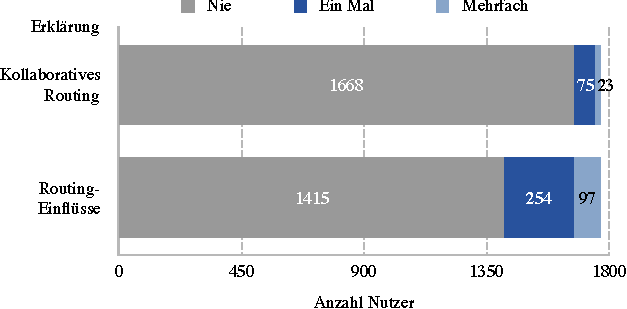
\includegraphics[width=0.9\textwidth]{contents/06_model_evaluation/02_evaluation/res/explanation_results_clicked.pdf}
    \caption{Anzahl der Nutzer, die Erklärungen erfasst haben}
    \label{fig:explanation_results_clicked}
\end{figure}


\autoref{fig:evaluation_explanation_demand_qualitative} zeigt die Bewertung der Studienteilnehmer des Quasi-Experiments in Bezug auf deren Bedarf für die Erklärungen.

In \autoref{fig:explanation_results_clicked} kann man erkennen, dass etwa 5\% der Nutzer auf die Erklärung zum kollaborativen Routing geklickt haben. Allerdings sagen wie in \autoref{fig:evaluation_explanation_demand_qualitative} zu erkennen ist drei von vier Teilnehmern des Quasi-Experiments, dass die die Erklärung benötigt haben. Folglich herrscht eine Diskrepanz zwichen dem wirklichen Bedarf und den \textit{End Usern} des Feld Tests, die die Erklärung angefordert haben. Insbesondere haben im Quasi-Experiment zwei der Teilnehmer angegeben, die Erklärung sich auch mehrfach anzusehen.

\begin{figure}[htb!]
    \centering
    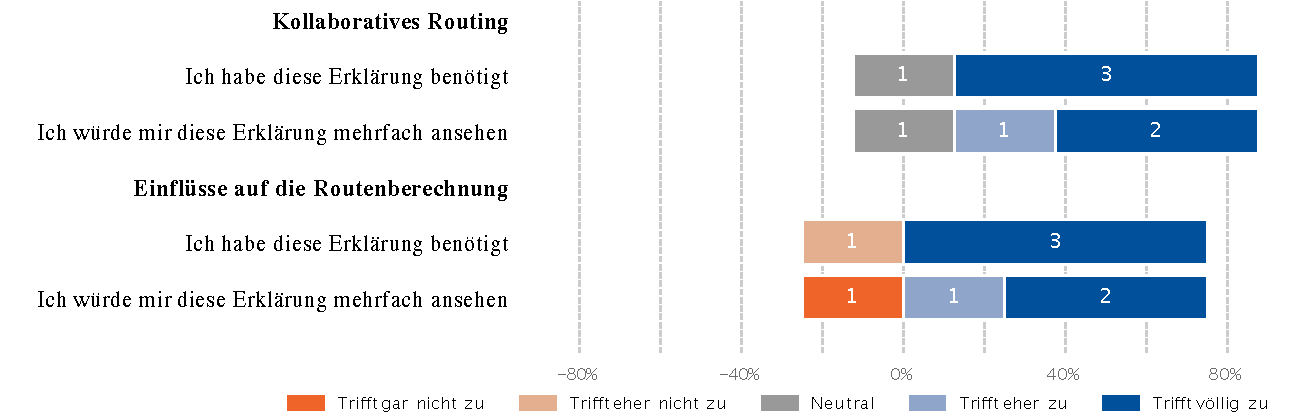
\includegraphics[width=\textwidth]{contents/06_model_evaluation/02_evaluation/res/qualitativeFeedback-evaluation_explanation_demand_qualitative.pdf}
    \caption{Subjektive Einschätzung des Bedarfs der Erklärungen}
    \label{fig:evaluation_explanation_demand_qualitative}
\end{figure}

Betrachtet man im Gegensatz dazu die gleichen Daten für die Erklärung zu den Einflüssen auf die Routenberechnung fällt auf, dass etwa 20\% der Teilnehmer des Feldtests sich die Erklärung angesehen haben, wie in \autoref{fig:evaluation_explanation_demand_qualitative} zu sehen aber, sowohl weniger Teilnehmer angegeben haben, dass sie die Erklärung benötigt haben als auch sich mehrfach ansehen würden als bei der Erklärung zum kollaborativen Routing. Ein Erklärungsversuch kann durch die Aussage eines Teilnehmers am Quasi-Experiment getätigt werden. Dieser sagte, dass die Zahl, auf die für die kollaborative Routing Erklärung geklickt werden müsse, zum Teil klar ist und nicht direkt offensichtlich ist, dass sich dorthinter die ALgorithmuserklärung befinde. Außerdem hat eine Teilnehmerin hinzugeügt, dass die Frage \glqq Wie ist meine Roue entstanden?\grqq{}, über welche die Erklärung zu den Routingeinflüssen erreichbar ist neugieriger macht.

Aus diesen freien Aussagen und dem Gegensatz zwischen den benötigten Erklärungen und den wirklich angeforderten, kann folglich abgeleitet werden, die Erklärung zum kollaborativen Routing offensichtlicher zu erreichen sein sollte. Die Idee eines weiteren Teilnehmers war, dass es Möglich sein sollte, diese Erklärung über den Dialog \glqq Trete Schwarm bei...\grqq{} erreichen zu können. Dies ist der Dialog, der zu sehen ist, während \textit{NUNAV Navigation} die erste Route während der Nutzung lädt.

Außerdem kann es dadurch, dass nur bis zu 20\% der \textit{End User} in der Feldstudie die Erklärungen gelesen haben, sein, dass die Auswirkungen auf andere Qualitätsmerkmale in der Studie nicht im signifikanten Bereich lagen. Zumindest für die Erklärung zum kollaborativen Routing ließe sich dies anhand der Aussagen der Teilnehmer des Quasi-Experiments durch einen versserten Weg, um zur Erklärung zu gelangen, ggf. steigern und sollte in einer zweiten Iteration getestet werden.



\subsubsection{Nützlichkeit der gegebenen Erklärungen}

\autoref{tab:explanation_results_clicked} zeigt die Bewertung als \glqq Hilfreich\grqq{} oder \glqq Nicht hilfreich\grqq{} durch die Nutzer. Allerdings sind die Hilfe-Artikel auch über andere Wege erreichbar, wodurch Bewertungen nicht nur von Nutzern kommen, die über die NUNAV-App dort hingeleitet wurden.

\begin{table}[htb!]
    \centering
    \begin{tabular}{p{.5\textwidth}p{.15\textwidth}p{.25\textwidth}}
        \hline
        Artikel & Hilfreich & Nicht Hilfreich \\
        \toprule
        Kollaboratives Routing & 76 & 9 \\
        Einflüsse auf die Routenberechnung & 209 & 32 \\
        \bottomrule
    \end{tabular}
    \caption{\textit{Usefulness} der Hilfe-Center-Artikel}
    \label{tab:explanation_results_clicked}
\end{table}

\begin{figure}[htb!]
    \centering
    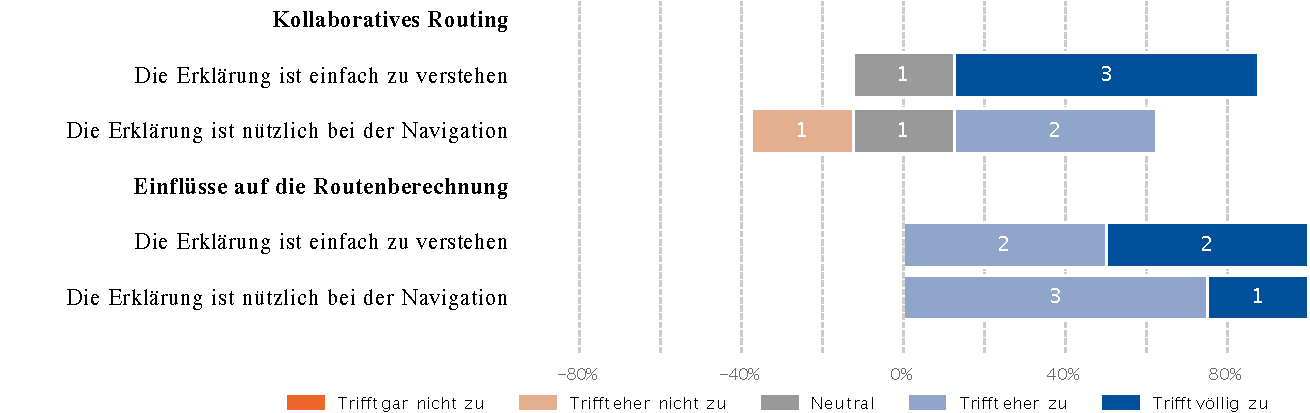
\includegraphics[width=\textwidth]{contents/06_model_evaluation/02_evaluation/res/qualitativeFeedback-evaluation_usefulness_qualitative.pdf}
    \caption{Subjektive Einschätzung des Bedarfs der Erklärungen (Anzahl der jeweiligen Bewertung pro Aussage)}
    \label{fig:evaluation_usefulness_qualitative}
\end{figure}

\newpage

\subsubsection{Erklärung: Kollaboratives Routing}

\begin{figure}[htb!]
    \centering
    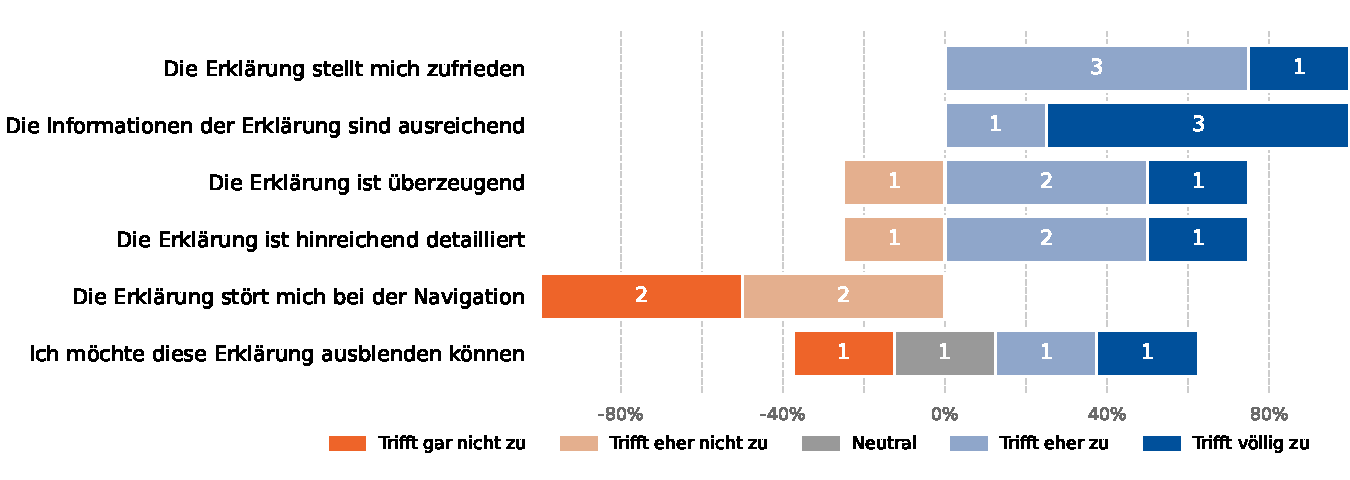
\includegraphics[width=\textwidth]{contents/06_model_evaluation/02_evaluation/res/qualitativeFeedback-01_collaborative_routing_short.pdf}
    \caption{Anzahl der jeweiligen Bewertung pro Aussage für die Erklärung zu kollaborativem Routing}
    \label{fig:01_collaborative_routing_short}
\end{figure}

\subsubsection{Erklärung: Einflüsse auf die Routenberechnung}

\begin{figure}[htb!]
    \centering
    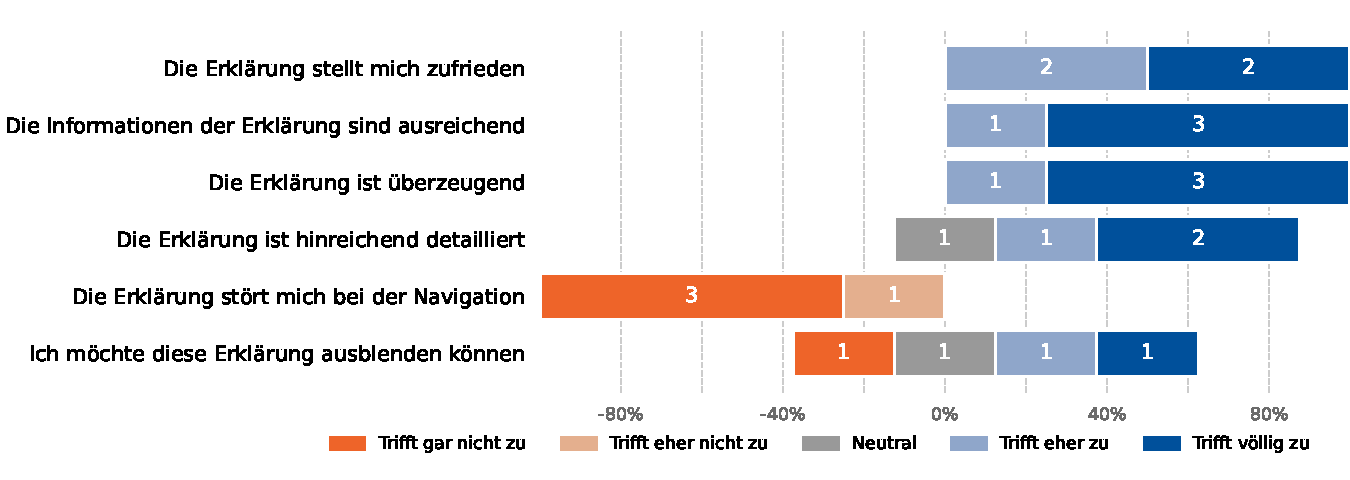
\includegraphics[width=\textwidth]{contents/06_model_evaluation/02_evaluation/res/qualitativeFeedback-02_collaborative_algorithm_short.pdf}
    \caption{Anzahl der jeweiligen Bewertung pro Aussage für die Erklärung zu Einflüssen auf die Routenberechnung}
    \label{fig:02_collaborative_algorithm_short}
\end{figure}


\subsubsection{Erklärung: Verkehrsaufkommen}


\subsubsection{Erklärung: Positionsungenauigkeiten}